\chapter{基于PID控制思想的码率自适应算法}

在实际网络环境中,带宽波动是不可避免的。对于一个视频流媒体系统而言,只有根据带宽变化来自适应地调整发送码率才能为用户提供更好的服务。在上一章中,我们通过可伸缩视频的码流截取,使得码率能够调整;在本章中,我们主要关注如何调整。由于视频码率与视频质量一般来说是直接相关的(高码率对应高质量),调整码率也就是调整所传送视频的质量。因此,本章所解决的问题又被称为质量控制问题。我们将基于经典控制实践中的PID思想,设计一个综合考虑带宽的历史状况、当前状态和未来趋势的码率自适应算法,从而提高发送视频的总体质量和平滑度。

\section{PID控制器简介}

PID控制器\footnote{http://en.wikipedia.org/wiki/PID\_controller}是一个在工业控制系统中常用的闭环反馈控制器。PID控制中的两个重要概念是过程变量和控制目标。过程变量代表着系统当前的状态,而控制目标是系统希望达到的理想状态。PID控制的基本思想就是根据过程变量和控制目标之间的误差来确定一个控制输出,该输出反馈作用到系统以最小化上述误差。

PID控制器的控制输出一般如下定义:
\begin{equation}
\label{eq:pid-output}
u(t) = {K_p} \cdot e(t) + {K_i} \cdot \int_0^t {e(\tau )d\tau }  + {K_d} \cdot \frac{d}{{dt}}e(t) \: ,
\end{equation}
其中$e(t)$指代过程变量与控制目标在时刻$t$的误差,$K_p$、$K_i$、$K_d$是三个可调参数,依次称为比例增益、积分增益和微分增益。公式(\ref{eq:pid-output})的结果通过某种方式来影响系统状态,使得过程变量朝着控制目标变化。

作为一个灵活有效的控制技术,PID可以被用来解决各种各样的控制问题\supercite{Wong2004}\supercite{Li1999}。在本文的工作中,我们基于它设计了一个码率自适应算法,用来控制视频流媒体中的视频质量。

\section{基于PID的码率自适应}

本节首先介绍质量等级的概念,将视频流媒体中的视频质量和码率值离散化,接着定义在所提出的码率自适应算法中用到的过程变量及其控制目标。之后,我们详细解释控制模型和算法流程,并简要讨论PID参数的选取和调优。

\subsection{质量等级划分}

视频质量或码率是一个连续的值,以任意的精度来控制或调整它是不现实的。因此,我们首先提出一个质量层级的概念来离散化视频质量和码率。当需要调整时,我们只是增加或减少质量等级。每一个质量等级对应一个确定的码率。高等级对应高码率,反之亦然。有多少个质量等级以及它们跟具体码率值如何对到应可以根据实际需求来确定。质量等级越多,系统就能越精细地调整码率来适应带宽变化。如绪论中所说,用多码流实现的自适应流媒体系统只能提供有限的几个质量等级,而基于可伸缩视频编码的流媒体系统能够以更高的精度来定义质量等级。

\subsection{过程变量和控制目标}

在本文所提出的质量控制算法中,所选取的过程变量称为“实际与检测间隔比”。下面介绍其具体定义。

\begin{figure}[h]
	\centering
	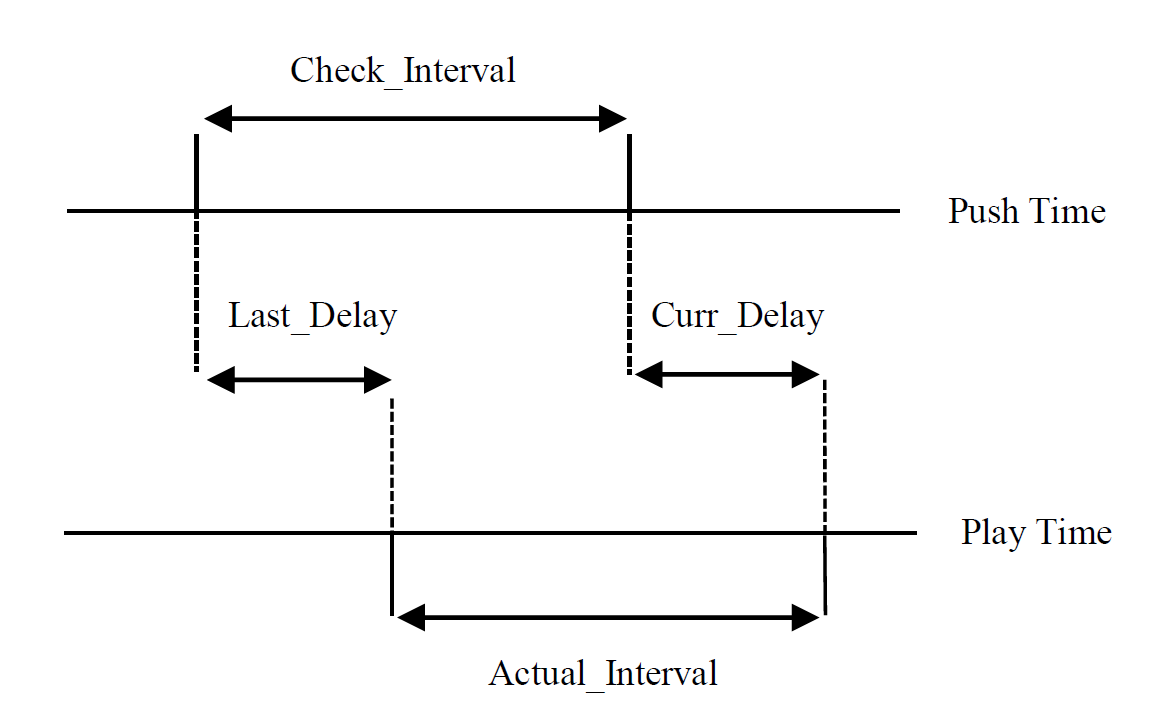
\includegraphics[width = 0.9\linewidth]{figures/Intervals.png}
	\caption{达尔文流媒体服务器中的两个时间线 \label{fig:intervals}}
\end{figure}

在达尔文流媒体服务器中,有两个时间线非常重要。第一个是推送时间线(push time),也就是视频数据包被推送到缓冲区的时间;第二个是播放时间线(play time),也就是数据包应该在播放中被显示的时间(通常记作该数据包的PTS)。这两个时间线的关系如图\ref{fig:intervals}所示。服务器程序会定时检测这两个时间线,并根据数据包的延迟来决定是否需要调整发送的视频质量。图\ref{fig:intervals}中的两个间隔,即检测间隔(check interval)和实际间隔(actual interval),值得我们注意。在理想情况下,每次检测间隔中服务器推送的数据量应该恰好能实际播放等于检测间隔的一段时间,也就是\textit{actual\_interval} = \textit{check\_interval}。如果实际间隔小于检测间隔,说明这段时间内推送了较少的数据,推送数据变慢很可能是带宽有所下降。反过来,如果实际间隔大于检测间隔,说明这段时间内推送了较多的数据,意味着网络条件良好且数据被快速推向客户端。这两个间隔的比值,也就是所谓的“实际与检测间隔比”,能够反映当前推送的速率是否与网络带宽相符。

“实际与检测间隔比”适合用作质量控制有三方面的原因。第一,这个比例直接对应着适合带宽的码率与当前传输的码率的比值,只需据此进行调整就可以准确地使码率符合带宽。第二,根据定义这个比例的理想值就是1,这就是算法的控制目标,无需再通过别的方法确定。第三,这个值在实际系统中便于计算,普适性较好。

\subsection{控制模型和算法描述}

在通常的PID控制器中,控制输出是用过程变量与控制目标之间的差值进行比例、积分、微分求取出来的。考虑到我们所选的过程变量是一个比例,且控制目标是1,本文对通常的PID控制器做了修改,提出了一个基于比例的模型。在这个模型中,过程变量直接被用来计算控制器输出,而且所有求差的运算都被适当的改为了求比例的运算,以保持模型的合理正确性,如下所示:

\begin{equation}
\label{eq:ut}
{u_t} = {K_p} \cdot E_p^t + {K_i} \cdot E_i^t + {K_d} \cdot E_d^t ,
\end{equation}

\begin{equation}
\label{eq:ep}
E_p^t = \frac{{actual\_interva{l_t}}}{{check\_interva{l_t}}} ,
\end{equation}

\begin{equation}
\label{eq:ei}
E_i^t = \frac{{long\_actual\_interva{l_t}}}{{long\_check\_interva{l_t}}} ,
\end{equation}

\begin{equation}
\label{eq:ed}
E_d^t = E_p^t/E_p^{t - 1} ,
\end{equation}

\begin{equation}
\label{eq:long-actual}
long\_actual\_interva{l_t} = \sum\limits_{\tau = {T_l}}^t {actual\_interva{l_\tau}} ,
\end{equation}

\begin{equation}
\label{eq:long-check}
long\_check\_interva{l_t} = \sum\limits_{\tau = {T_l}}^t {check\_interva{l_\tau}} .
\end{equation}

在公式(\ref{eq:ut})中:$K_p$、$K_i$、$K_d$分别表示比例部分、积分部分、微分部分的可调参数;$E_p^t$、$E_i^t$、$E_d^t$则对应各部分在第t次检测时的值,它们的定义如公式(\ref{eq:ep})至(\ref{eq:long-check})所示;控制器输出$u_t$将用来计算适合当前带宽的码率,并据此选择要传送的质量等级。

在公式(\ref{eq:long-actual})和(\ref{eq:long-check})中,$T_l$代表上一次质量等级改变的时间。按照理论定义,积分部分应该从系统启动开始记录,但在实际环境中,网络带宽有可能变动非常大,如果积分部分记录累积太长时间将不适合反映当前的网络条件,从而减缓调整质量的决策。因此这里采用了一个折衷,选择从上一次质量等级变化的时间开始计算积分部分。

这个基于比例的模型对于所选的过程变量和控制目标比通用模型更加简单有效。而且,在该模型中,当三个参数进行归一化处理后,控制器输出具备明显直观的意义。从公式(\ref{eq:ep})至(\ref{eq:long-check})容易看出,$E_p^t$、$E_i^t$、$E_d^t$这三个值都是在1附近波动的比值;而根据公式(\ref{eq:ut}),控制器输出$u_t$可以被视作这三个比值的加权平均(三个参数作为权值)。因此,$u_t$也是一个在1附近的比值,它对应着适合当前带宽的码率与当前发送码率的关系。换句话说,如果$u_t$大于1,那么控制器决定当前发送码率需要增加;反之,如果$u_t$小于1,意味着控制器认为当前发送码率需要减小。用$u_t$作为一个乘子来调整当前发送的码率,我们就能控制流媒体系统符合带宽的变化。

本文提出的码率自适应算法描述如Algorithm\ref{algo:control}所示。相比于其他的调度策略,这个基于PID的自适应算法具有以下几个优点。首先,该算法不仅仅依据当前状态或者固定时间点的信息来做决策,因此质量调整可以在任何合适的时间发生。其次,因为PID模型(微分部分)在某种程度上考虑了对未来的预测,该算法能够判断带宽在未来一段时间内是否会变得足够大或足够小,因此能避免一些不必要的调整。最后,该算法并不一定一次只调整一个质量等级,这就使得当带宽剧烈下降时能够快速下调质量以保证流畅播放,而当系统启动时能够快速上调质量以使用户尽早收到更清晰的视频。

\begin{algorithm}
	\caption{基于PID的码率自适应算法}
	\label{algo:control}
	\begin{algorithmic}
		\STATE 准备发送数据包
		\STATE check\_interval = curr\_time -- last\_check\_time
		\STATE actual\_interval = curr\_media\_time -- last\_check\_media\_time
		\STATE long\_check\_interval += check\_interval
		\STATE long\_actual\_interval += actual\_interval
		\STATE 根据公式(\ref{eq:ep}) - (\ref{eq:ed})计算$E_p^t$、$E_i^t$、$E_d^t$的值
		\STATE output = ${K_p} \cdot E_p^t + {K_i} \cdot E_i^t + {K_d} \cdot E_d^t$
		\STATE new\_bitrate = output * curr\_bitrate
		\STATE new\_level = get\_level(new\_bitrate, bitrate\_of\_level[])
		\IF {质量等级变化}
		\STATE long\_check\_interval = 0
		\STATE long\_actual\_interval = 0
		\STATE curr\_bitrate = bitrate\_of\_level[new\_level]
		\ENDIF
		\STATE 根据新的质量等级发送数据包
	\end{algorithmic}
\end{algorithm}

\subsection{参数选取与调优}

与工业界的其他PID控制系统一样,本文提出的算法中三个参数的选取也是跟具体实现相关的。大多数情况下,为取得最优的效果,需要手动试错调节。每个参数对系统的不同方面产生影响,知道这些影响有助于进行参数选取。一般来说,PID控制器中的比例部分会影响系统的稳定性。如果比例增益$K_p$过高,系统容易变得不稳定。但是,太低的$K_p$又会导致过长的上升时间,使系统响应迟缓。积分部分除了能消除稳态误差,还能加速过程变量向控制目标的变化。这意味着,增大$K_i$能减小上升时间,提高系统的响应速度。但是,积分部分会累积过去一段时间的误差,使过程变量容易超出目标值(即超调),因此过大的$K_i$也会导致系统不稳定。上述这些隐患都能通过微分部分来校正。微分部分通过预测系统行为,具有减小超调、提高稳定性的双重效果。但是微分部分的特点是对误差分成敏感,也正是因为此,工业实践中微分增益$K_d$通常都设置的比较低。

本文采用了经典的Ziegler--Nichols方法\supercite{Ziegler1942}来进行参数选取。该方法首先把积分和微分参数设为0,调节比例参数$K_p$到系统开始震荡时的值$K_u$,假设震荡周期为$T_u$,那么设置$K_p = 0.6K_u$、$K_i = 2K_u/T_u$、$K_d = K_u \cdot T_u/8$。再将$K_p$、$K_i$和$K_d$进行归一化,就得到最终的参数:$K_p = 0.22$,$K_i = 0.73$,$K_d = 0.05$。在这样的参数配置下,由本文提出的算法所控制的流媒体系统是稳定的,而且能够很快开始适应带宽的变化,具体参见下一节中的实验结果。

\subsection{扩展应用到直播系统}

PID控制思想具有很强的扩展性,除了上述在达尔文流媒体点播中的应用,我们还将其用在了直播系统中。本小节对这一扩展应用进行介绍,重点是说明点播系统与直播系统的不同之处,以及如何选取合适的过程变量和控制目标。

在有些视频直播系统中,视频内容由服务器或者与服务器通过局域网连接的设备生成,在这种情形下,视频直播和视频点播具有很多共同点。在直播中服务器将动态生成的视频数据发送给客户端,和点播最主要的区别在于传输速率不能超过视频数据生成速率,因此当所有生成的数据都传输之后,客户端需要等待下一个数据片段就绪\supercite{Thang2014}。而在如今十分火热的用户生成内容(UGC)直播模式下,服务器本身不充当初始的内容产生方,在其他设备上持续生成的视频内容经过不确定且不可忽略的延迟传输到中转服务器。目前已经分成普及的智能手机成为了理想的内容产生方和接收方。图\ref{fig:07}展示了通用的手机视频直播系统的主要模块。集成了高效视频编码器的智能手机,将实时视频数据传输到接收服务器,在此同时,原始视频流被转码成多路具有不同码率的视频流。客户端可以通过当前网络环境选择最合适的码率,从服务器获取视频数据。

\begin{figure}[h]
	\centering
	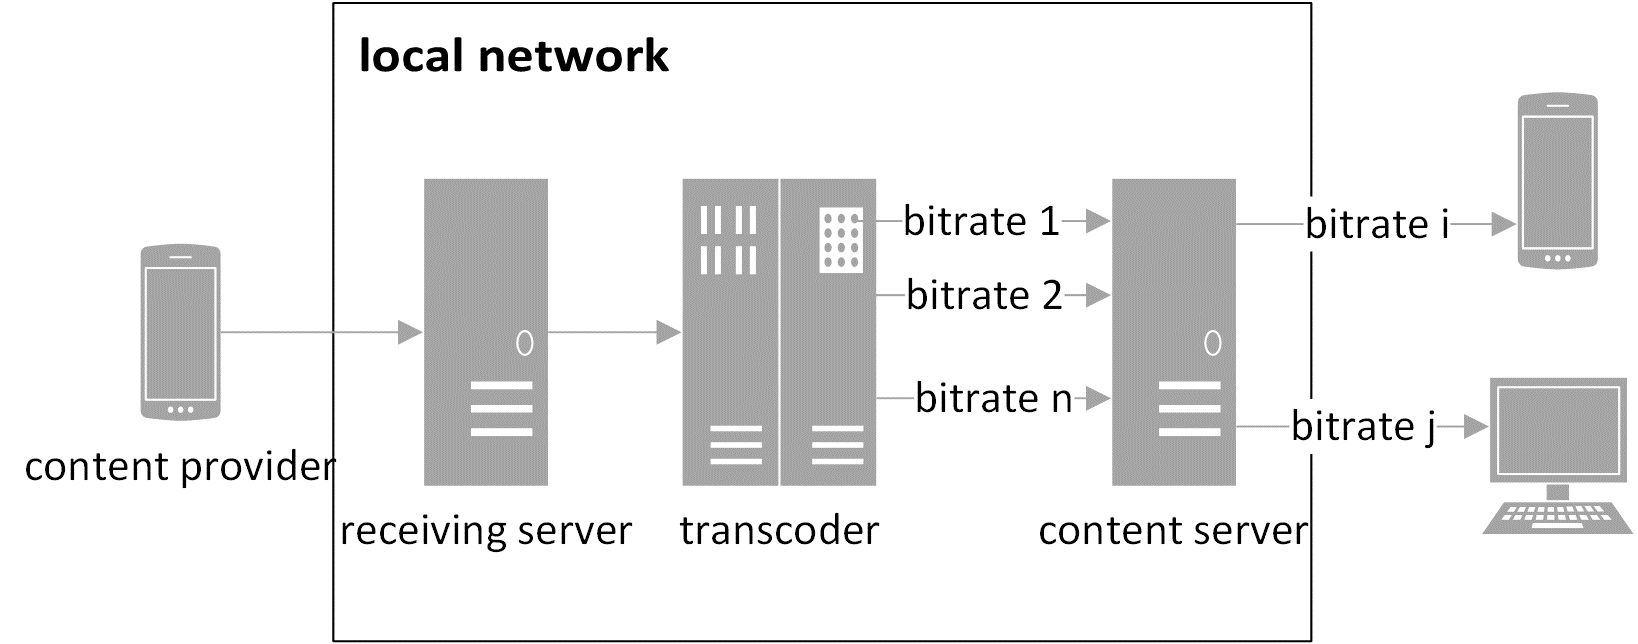
\includegraphics[width = 1.0\linewidth]{clip/07.png}
	\caption{通用的手机直播系统模型\label{fig:07}}
\end{figure}

为了提供高质量的直播视频流,内容产生方需要传输尽可能高码率的视频,这可能导致每个数据段传输时间过长,造成接收端的播放中断。而内容产生方在变化的网络状况下尽可能利用网络吞吐量传输高质量视频的同时保证接收端的流畅播放,是一个挑战。与此同时,延迟需要控制在一个可以接收的范围。我们在内容产生方设计了一个上传码率自适应控制器,这种方案能够应用于UGC的视频直播。

简单起见,我们假设服务器具有快速的内部操作,同时接收端通过稳定高效地网络与服务器进行连接,这意味着服务器和接收端的视频流与内容产生方和服务器的视频流保持同步。这个假设对我们的研究重点没有影响。我们将传输架构简化成如图\ref{fig:08}所示。内容产生方的编码器将输入视频压缩之后传递给基于TCP的应用层协议。经过各层协议的封装,数据被传递到网络进行实际传输。在接收端经过一个逆向过程之后,数据输入到解码器进行解码,然后在播放器中进行渲染。与此同时,在发送方的自适应控制器每隔特定的周期对传输信息进行检查,并采用后文将介绍的特定的策略对编码器参数进行调整。

\begin{figure}[h]
	\centering
	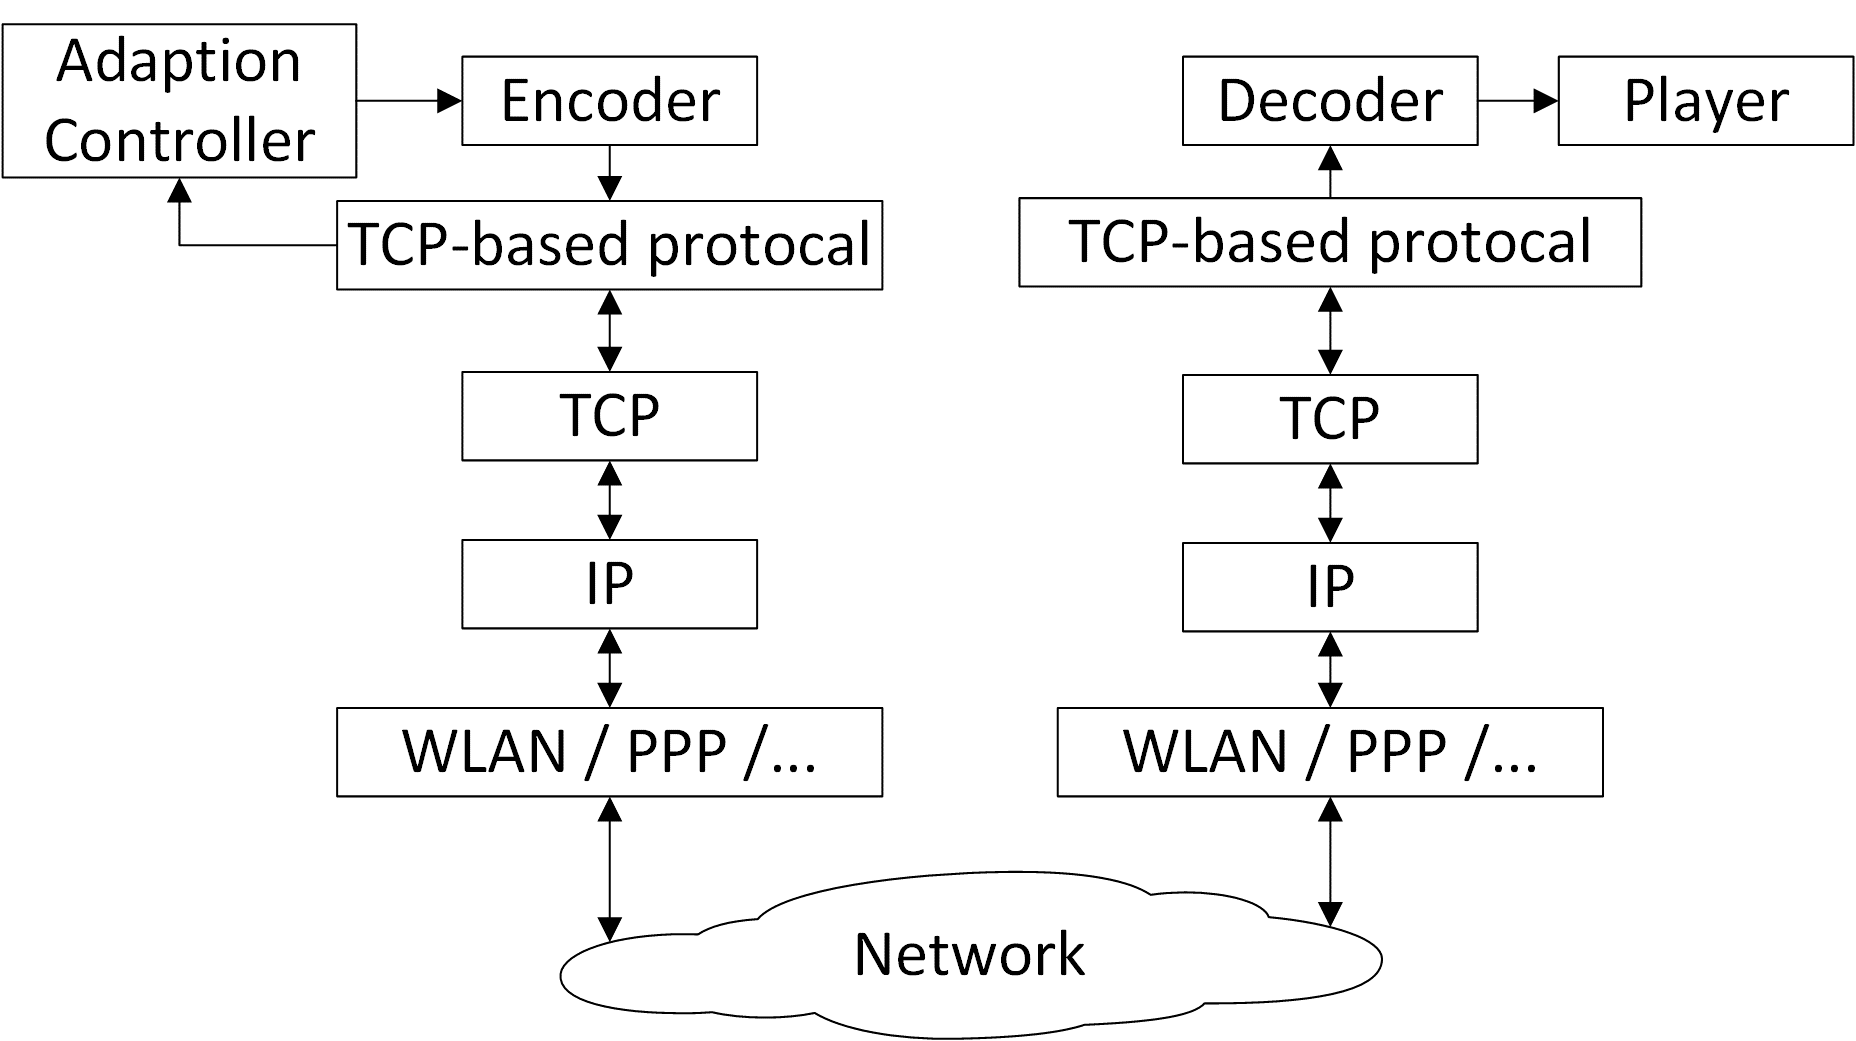
\includegraphics[width = 1.0\linewidth]{clip/08.png}
	\caption{简化直播系统传输架构\label{fig:08}}
\end{figure}

使用PID进行码率自适应的关键在于选取一个能够反映传输状况的过程变量。基于TCP的直播系统在传输过程中有四个缓冲区,分别是应用层发送缓冲区(ASB)、TCP发送缓冲区、TCP接收缓冲区、播放缓冲区(PB)。其中对内容产生方最重要的信息是ASB内的数据长度,记为择$S_{ASB}(t)$(在时刻$t$的值),它能够直接反映视频码率和吞吐量之间的匹配情况。当视频码率高于当前的吞吐量时,该缓冲区内的数据长度趋向于增大,否则保持相对稳定或者减小为0。理想状况下,它首先应该是一个大于0的值,以保证接收方播放不中断;其次它不应该太大,否则意味着发送码率太高。所以,我们选择$S_{ASB}(t)$作为系统的过程变量,而选择一个接近0的常量$\varepsilon$作为控制目标。

然而,如果网络吞吐量在一个小的范围频繁波动,将使得系统变量值不稳定而且相对随机,导致不必要的频繁的调整。为了消除这样的随机性,我们将过程变量的定义修改为$\overline{S_{ASB}(t)}$,它表示在时刻$t$之前的一个时间段$\tau$内$S_{ASB}(t)$的平均值。它可以表示为:
\begin{equation}
\label{eq:asb}
\overline{S_{ASB}(t)} = \dfrac{1}{\tau} \int_0^\tau {S_{ASB}(t)}\: .
\end{equation}

对于UGC直播应用来讲,由于发送的码流是实时生成的,所以调整码率时直接改变编码器参数以改变生成码率即可,不需要涉及码流截取等数据源端的操作。但是,质量等级的概念仍然需要,它在这里变成了改变码率的单位。控制模型可以直接采用原始PID中的做法,用过程变量和$\varepsilon$的差值来计算比例、积分、微分这几个部分。具体的算法流程以及三个PID参数的选取和调优与上一小节中的相同,这里不再详述。

\section{实验结果}

\subsection{用伸缩层组合定义的质量等级}

为了简单起见,在第一部分实验中,我们先用可伸缩视频内置的伸缩层级组合成质量等级来用于质量控制。该定义的基本思想是将视频码流中的数据包分成若干组。分组的依据是这个数据包所属的伸缩层,也就是储存在NALU头信息中的层ID字段。表\ref{tab:sub-stream}展示了组ID与层ID的对应关系。我们所用的测试码流含有3个质量层和3个时间层,因此其中的数据包被分为9个组。质量等级被定义为组ID不大于等级值的所有组的合集。例如,质量等级2含有组0到组2内的所有数据包,因此将包含所有的时间层,但只有质量基本层;质量等级5含有组0到组5,于是将进一步包括第一个质量增强层的数据包。类似这样,随着质量等级的升高,越来越多的增强层数据包被累积进来,视频质量逐渐提升;与此同时,码率也越来越高,因为更好的质量显然需要更高的码率。我们测试用的完整码流码率是1587kbps,对应着最高的质量等级。这样用伸缩层来构造质量等级可以不用额外的数据,只需解析码流中本来已经包含的层ID即可,实现起来比较简单。

\begin{table*}[h]
\centering
\caption{质量等级定义中组ID与层ID的对应关系}
\label{tab:sub-stream}
\begin{tabular}{c|*{8}{p{1.0cm}<{\centering}|}{p{1.0cm}<{\centering}}}
	\hline\hline
	  组ID   & 0 & 1 & 2 & 3 & 4 & 5 & 6 & 7 & 8 \\ \hline
	质量层ID  & 0 & 0 & 0 & 1 & 1 & 1 & 2 & 2 & 2 \\ \hline
	时间层ID & 0 & 1 & 2 & 0 & 1 & 2 & 0 & 1 & 2 \\ \hline
\end{tabular}
\end{table*}

\subsection{实验配置}

在我们的实验中用限速软件NetLimiter\footnote{http://www.netlimiter.com/}来模拟实际网络环境中的带宽情况。平均带宽的取值从400kbps到1400kbps,以100kbps的间隔递增。对于每个平均带宽值,通过在平均值基础上加随机干扰来模拟带宽波动。在带宽波动的情况下,流媒体系统在每种质量控制算法下各运行10分钟,并记录所发送的质量等级变化。所有质量等级的平均值作为视频质量的度量,而所有质量等级的方差作为质量平滑性的度量。这两个指标被用于不同算法的比较。比较中的基准算法是达尔文流媒体服务器中内置的包延迟反馈(packet delay feedback,简称PDF)算法。

接下来,我们展示各种质量控制算法的结果并进行分析比较。

\subsection{结果和分析}

为了分析PID控制模型各个部分的效果,我们首先只用比例部分和积分部分来进行了初步的测试实验。由于这两个部分各自对应当前的短期误差和积累的长期误差,我们分别称之为短期预测算法(short-term prediction,简称STP)和长期预测算法(long-term prediction,简称LTP)。图\ref{fig:performance-all}展示了这两种控制算法和基准算法的实验结果。可以看出,短期预测算法能取得最高的平均质量等级,但它的质量等级方差也是最高的。这正符合短期预测总是倾向于紧紧跟随带宽变化的特点。长期预测算法恰恰与之相反,保持了一个较低的质量等级方差,但也牺牲了一部分平均质量。虽然它的平均质量不如短期预测算法,但也超出了基准算法。

\begin{figure*}[t]
\centering
\subfloat[不同质量控制算法的质量等级均值]{
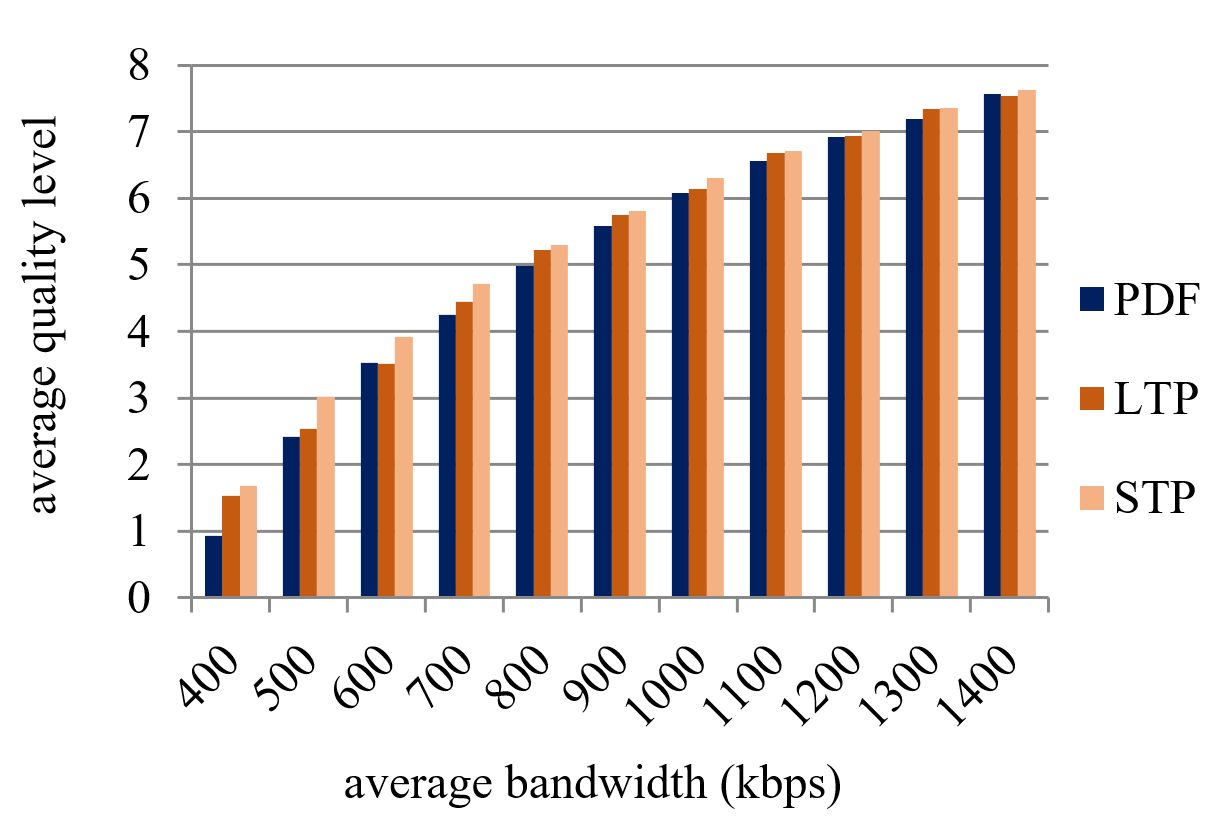
\includegraphics[width=0.5\textwidth]{figures/Quality-all.png}
\label{fig:quality-all}}
\subfloat[不同质量控制算法的质量等级方差]{
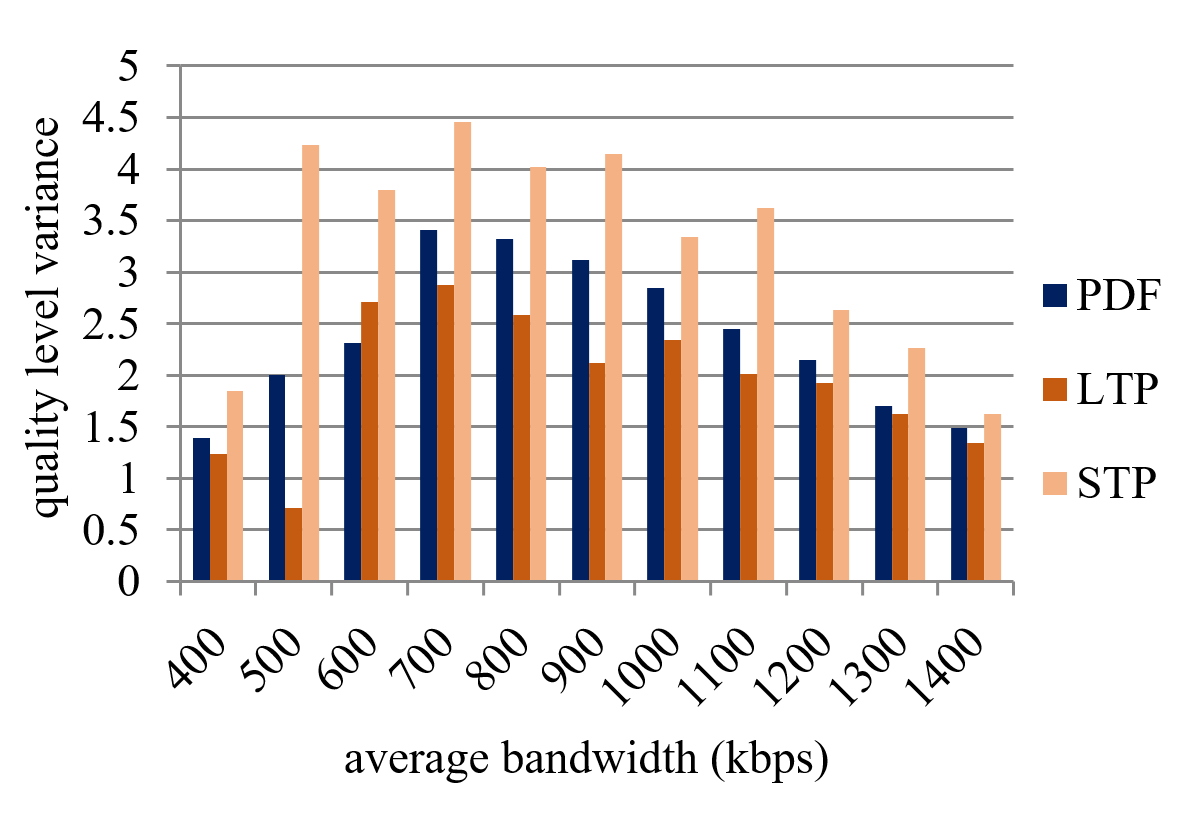
\includegraphics[width=0.5\textwidth]{figures/Variance-all.png}
\label{fig:variance-all}}
\caption{长/短期预测算法与达尔文服务器中的包延迟反馈(PDF)算法的比较}
\label{fig:performance-all}
\end{figure*}

\begin{figure*}[t]
\centering
\subfloat[PID和PDF算法的质量等级均值]{
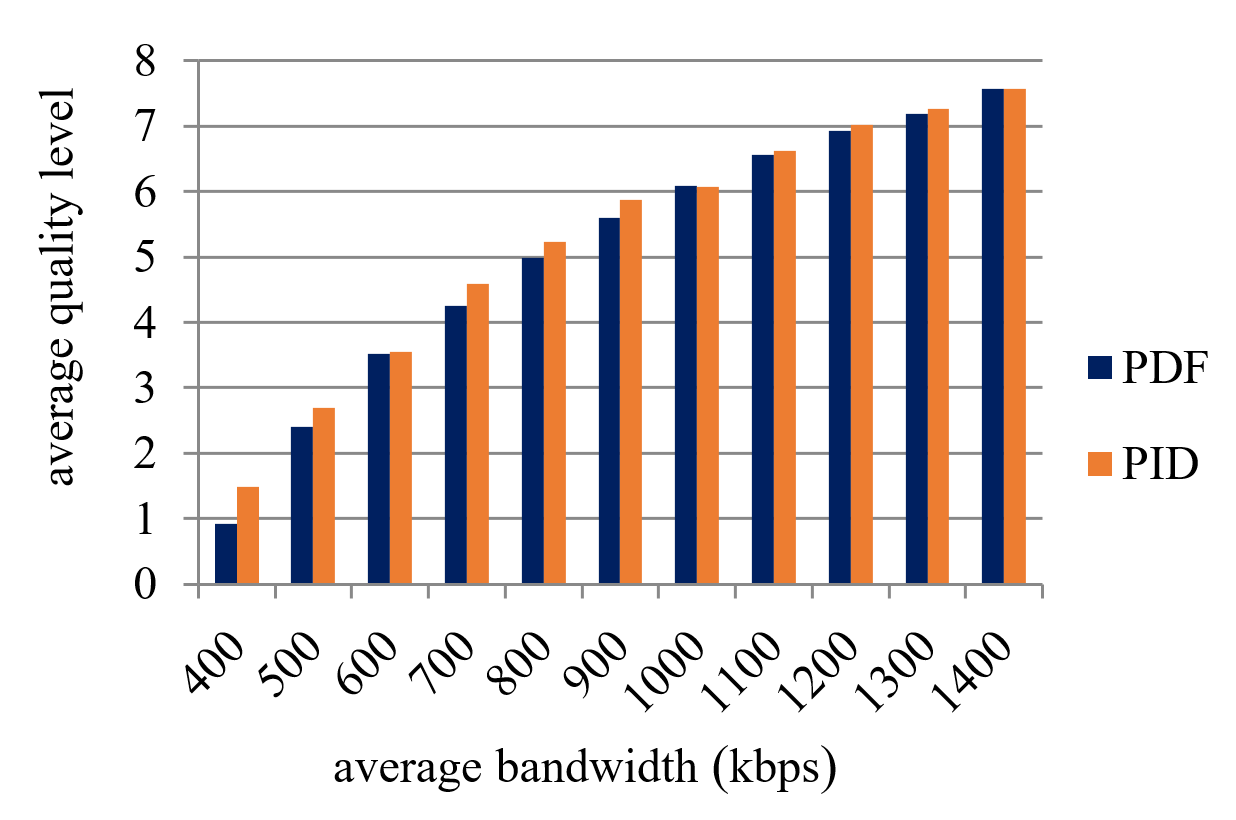
\includegraphics[width=0.5\textwidth]{figures/Quality-two.png}
\label{fig:quality-two}}
\subfloat[PID和PDF算法的质量等级方差]{
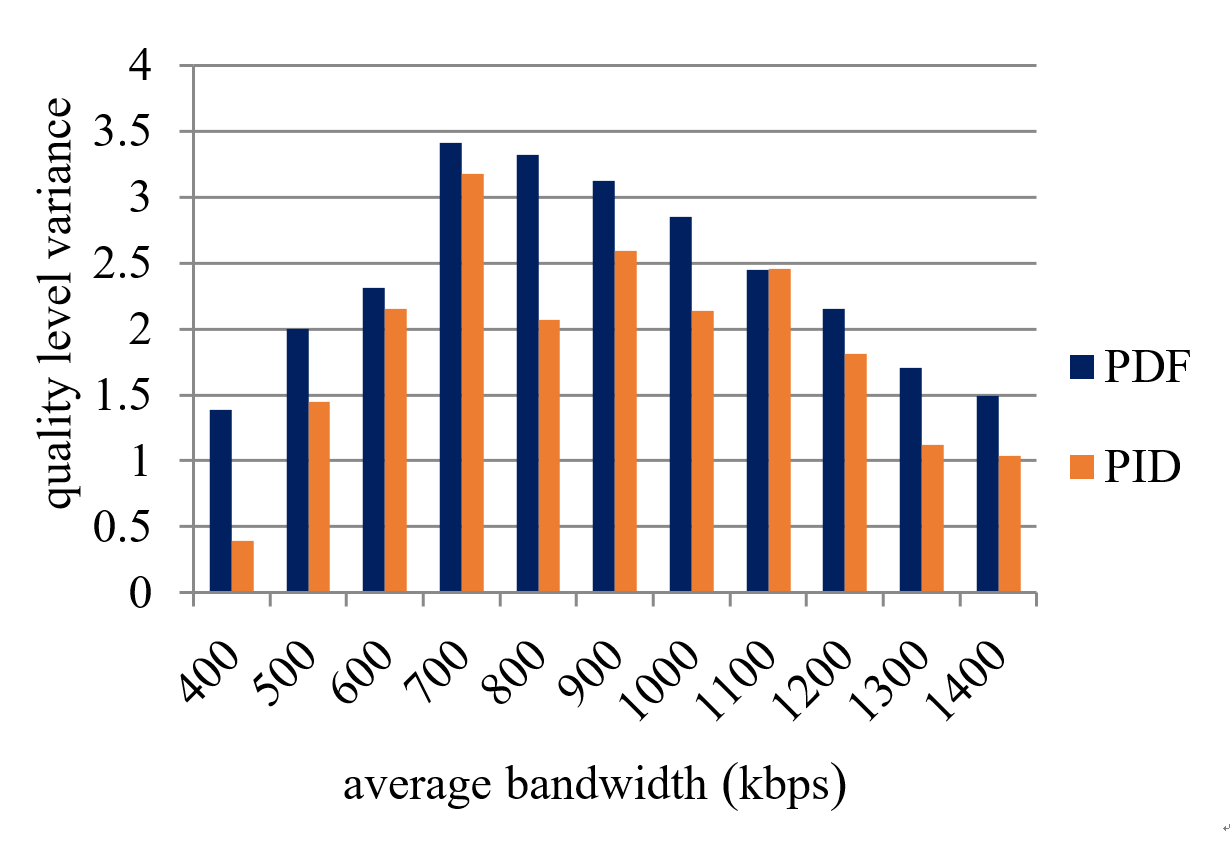
\includegraphics[width=0.5\textwidth]{figures/Variance-two.png}
\label{fig:variance-two}}
\caption{本文提出的PID控制算法与达尔文服务器中的包延迟反馈(PDF)算法的比较}
\label{fig:performance-two}
\end{figure*}

短期预测和长期预测算法有各自的局限性,完整的PID控制算法则既能降低质量波动又能提升平均质量。实验结果可参见图\ref{fig:performance-two}。可以看到,当与积分和微分相结合后,比例部分在短期预测算法中那样的激进效果已经弱化了。如图\ref{fig:variance-two}所示,PID算法取得了比PDF算法更低的质量波动。

表\ref{tab:improvement}列出了四种控制算法的定量比较数据,从中我们可以看出PID算法相比其他几种算法有明显的优势。与基准算法PDF相比,基于PID的质量控制算法取得了8.6\%的视频质量提升,同时将质量波动也降低了24.8\%。当带宽在平均值800kbps附近波动的时候,四种控制算法对应的视频质量等级变化情况如图\ref{fig:fluctuation}所示。从中我们可以明显观察到PID控制算法得到的视频质量更加平稳。

\begin{table*}[h]
\centering
\caption{不同质量控制算法与包延迟反馈算法的定量比较}
\label{tab:improvement}
\begin{tabular}[b]{p{4.2cm}<{\centering}|p{4.2cm}<{\centering}|p{4.2cm}<{\centering}}
\hline \hline
控制算法 & 质量等级均值的增长 & 质量等级方差的增长 \\ \hline
包延迟反馈 (PDF) & 0.0\% & 0.0\% \\ \hline
短期预测 (STP) & \textbf{+13.5\%} & +38.5\% \\ \hline
长期预测 (LTP) & +7.9\% & -17.2\% \\ \hline
PID控制 (PID) & +8.6\% & \textbf{-24.8\%} \\ \hline
\end{tabular}
\end{table*}

\begin{figure}
\centering
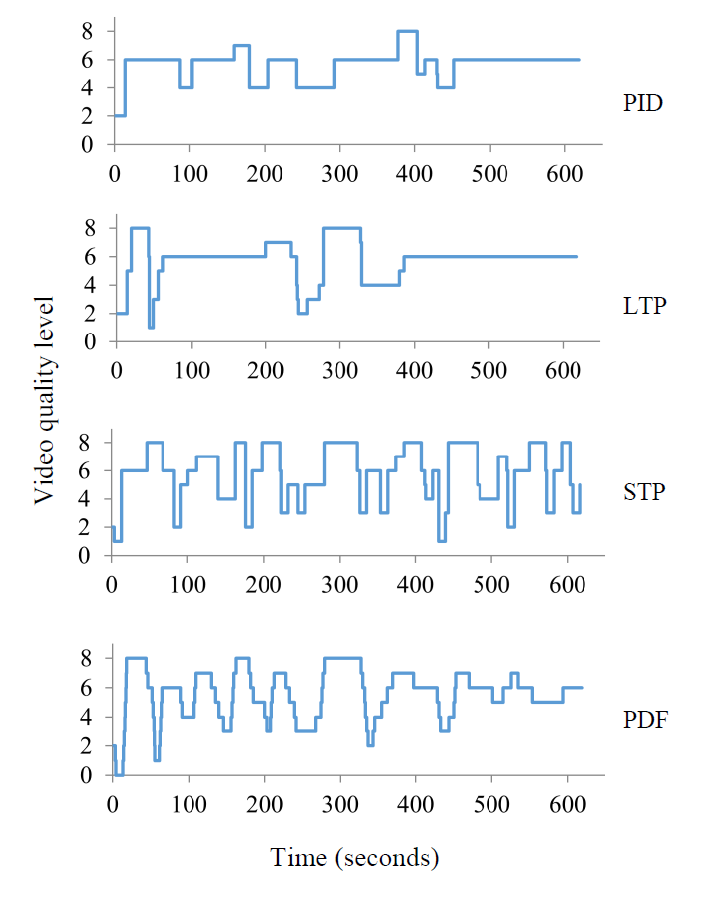
\includegraphics[width = 0.45\linewidth]{figures/Fluctuation.png}
\caption{不同质量控制算法下视频质量等级随时间的变化情况 \label{fig:fluctuation}}
\end{figure}

\subsection{与码流截取相结合的效果}

上面的实验直接用可伸缩视频中内置的伸缩层来构造质量等级,并没有结合本文前一章中提出的码流截取算法。实际的可伸缩视频流媒体系统中,当码率自适应算法给出一个适合传输的码率后,由码流截取方案根据这一码率限制截取出一个子流向客户端发送。本小节展示将本文提出的算法相结合的系统运行效果。

我们的比较对象是采用其内置的质量控制算法和JSVM基本码流截取方案的达尔文流媒体服务器。比较结果如图\ref{fig:fluctuation-psnr}所示。其中展示了带宽在400kbps、600kbps、800kbps和1000kbps附近波动时,所发送视频流的PSNR变化情况。可以看到,采用本文算法的系统性能要好于比较对象,体现在:一,成功避免了不必要的质量下降,例如图\ref{fig:Fluctuation-PSNR3}的350秒处和图\ref{fig:Fluctuation-PSNR4}的150秒处;二,能够维持一个相对更高的PSNR值,例如图\ref{fig:Fluctuation-PSNR1}的450秒附近和图\ref{fig:Fluctuation-PSNR2}的500秒附近。整个时间过程中的PSNR均值和方差在图\ref{fig:fluctuation-psnr}中也有列出,定量地证明了本文算法的优越性。例如,在图\ref{fig:Fluctuation-PSNR3}中,当带宽在800kbps波动时,采用本文算法的系统所传送视频的PSNR平均值为38.75dB,比比较对象高了0.83个dB,同时PSNR方差也由1.24降低到了0.69,意味着视频质量平滑性也更好。

\begin{figure*}[t]
\centering
\subfloat[带宽在400kbps附近波动:PSNR均值和方差在原始系统中是36.00和0.30,而在采用本文算法的系统中是36.50(提高了0.50)和0.23(降低了0.07)。]{
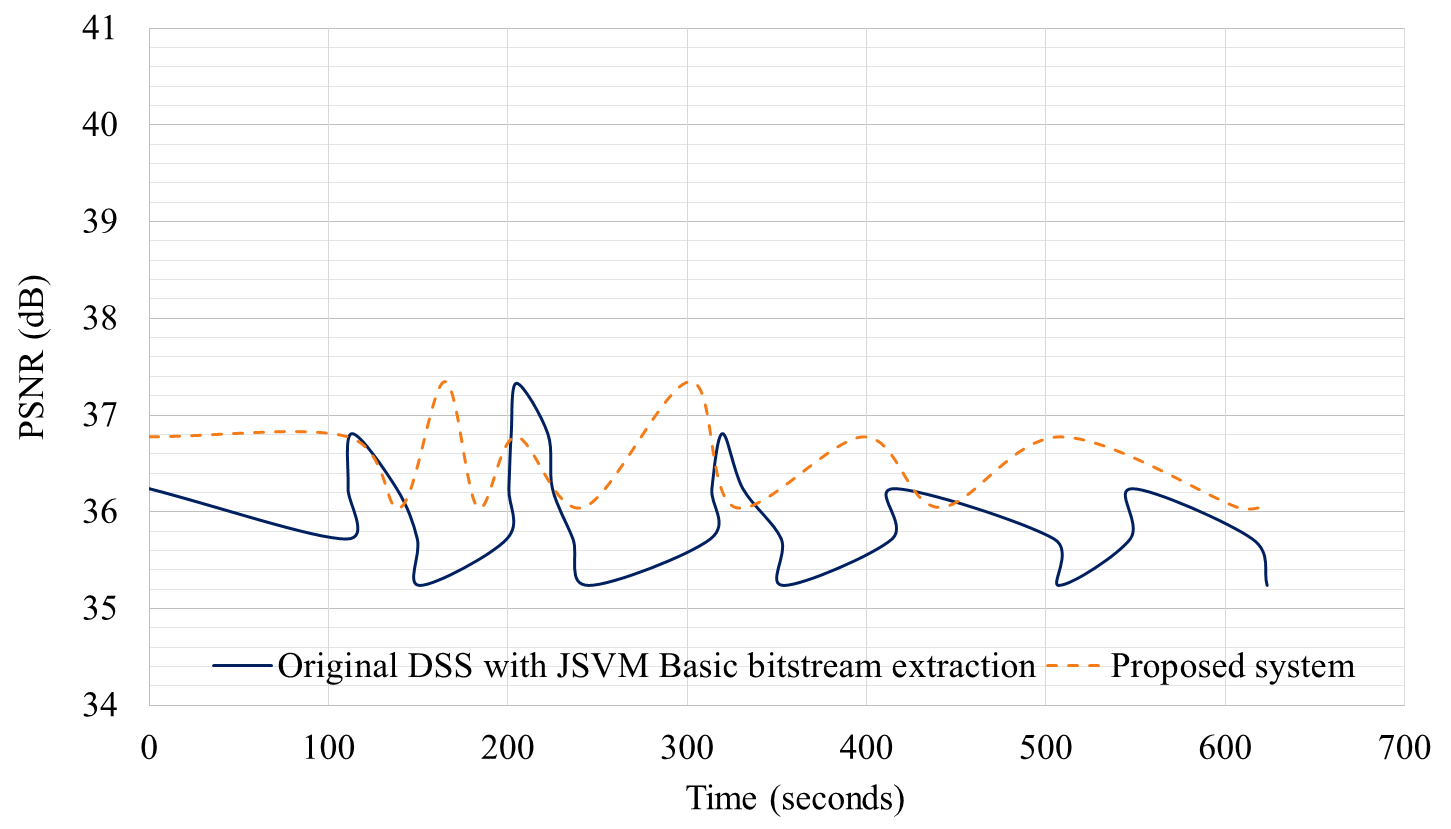
\includegraphics[width=0.47\textwidth]{figures/Fluctuation-PSNR1.png}
\label{fig:Fluctuation-PSNR1}}\hfill
\subfloat[带宽在600kbps附近波动:PSNR均值和方差在原始系统中是37.06和0.61,而在采用本文算法的系统中是37.32(提高了0.26)和0.33(降低了0.28)。]{
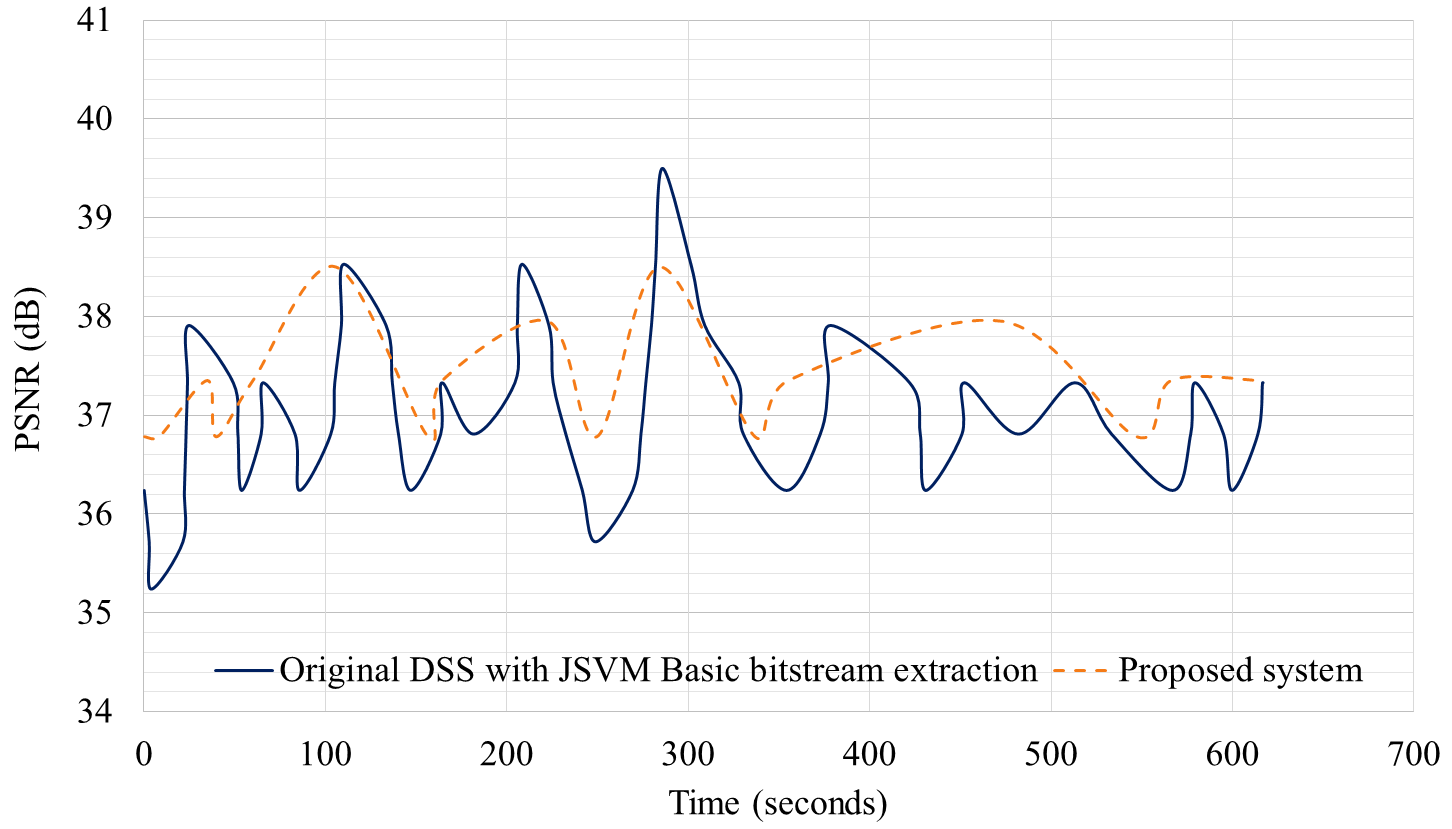
\includegraphics[width=0.47\textwidth]{figures/Fluctuation-PSNR2.png}
\label{fig:Fluctuation-PSNR2}}
\qquad
\subfloat[带宽在800kbps附近波动:PSNR均值和方差在原始系统中是37.92和1.24,而在采用本文算法的系统中是38.75(提高了0.83)和0.69(降低了0.55)。]{
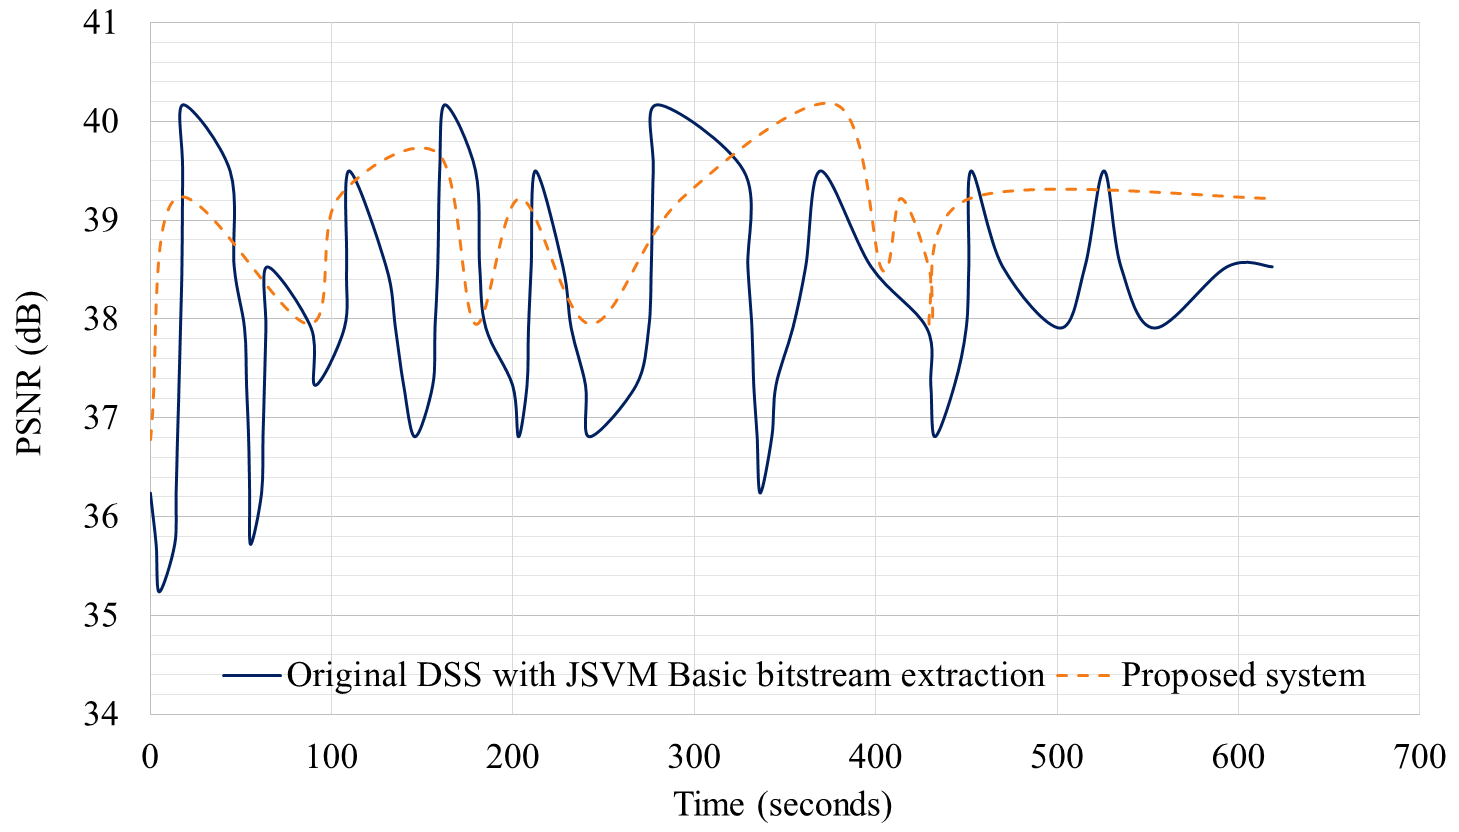
\includegraphics[width=0.47\textwidth]{figures/Fluctuation-PSNR3.png}
\label{fig:Fluctuation-PSNR3}}\hfill
\subfloat[带宽在1000kbps附近波动:PSNR均值和方差在原始系统中是38.28和1.30,而在采用本文算法的系统中是38.94(提高了0.66)和0.71(降低了0.59)。]{
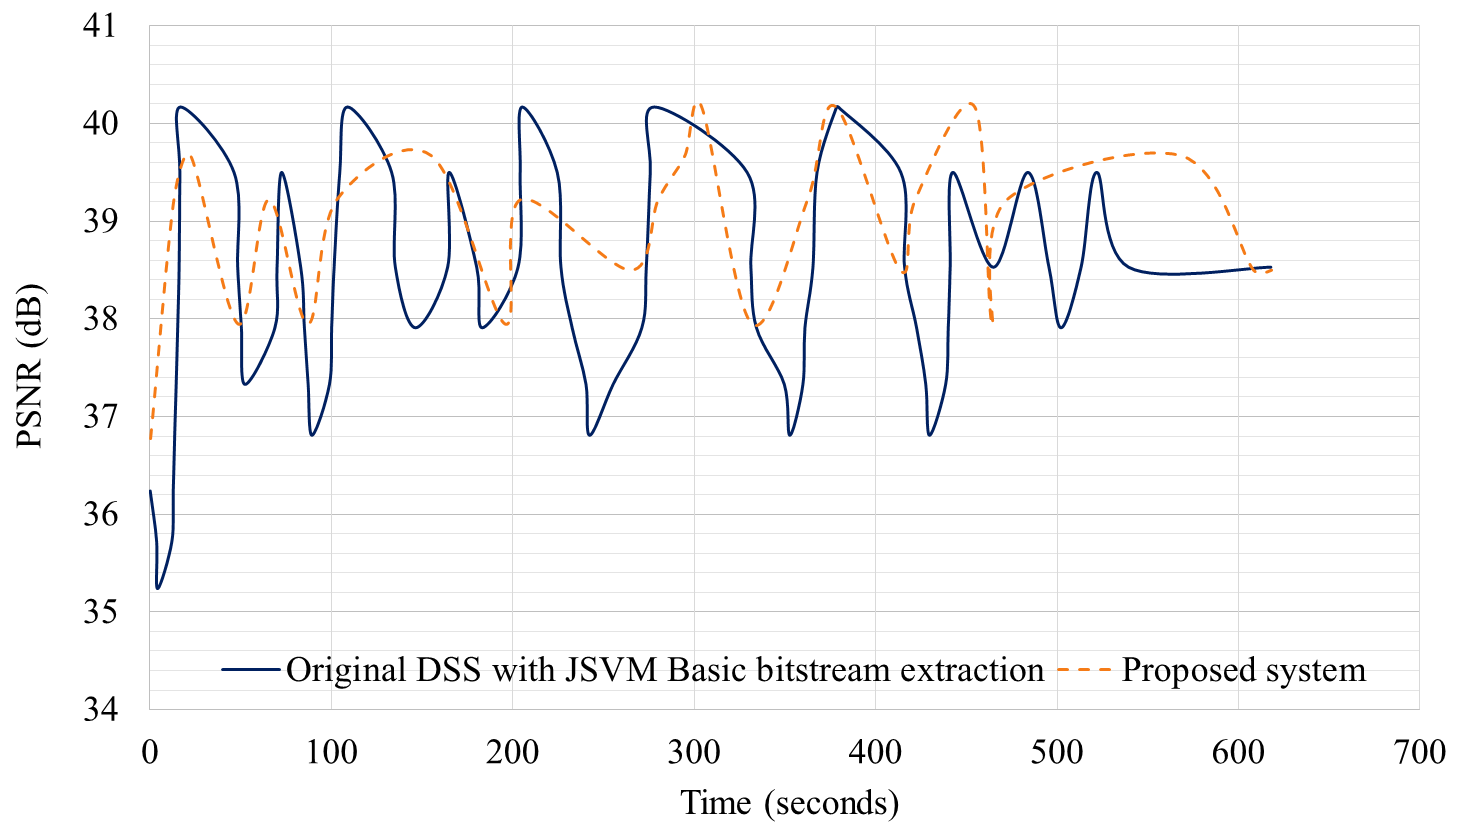
\includegraphics[width=0.47\textwidth]{figures/Fluctuation-PSNR4.png}
\label{fig:Fluctuation-PSNR4}}
\caption{不同流媒体系统所发送视频的PSNR随时间的变化情况
\label{fig:fluctuation-psnr}}
\end{figure*}


\subsection{用在直播系统中的效果}

为了对基于PID的直播系统内容发送码率自适应方法进行测试,我们实现了一个基于TCP的手机视频直播系统。我们选择业界已经广泛使用的RTMP协议作为应用层流媒体协议,具体实现采用了第三方开源的代码库librtmp\footnote{http://rtmpdump.mplayerhq.hu/librtmp.3.html}。我们用nginx-rtmp-module\footnote{https://github.com/arut/nginx-rtmp-module}帮助完成了中转服务器的搭建。我们采用了开源软件x264\footnote{http://www.videolan.org/developers/x264.html}作为视频编码器。我们在Android平台上实现了内容产生和上传的程序,集成了我们提出的自适应码率控制算法,并采用开源播放器ffplay\footnote{https://ffmpeg.org/}作为接收方,它可以播放RTMP协议的流媒体并对播放缓冲区长度进行预设。我们通过动态改变内容产生方所连接的路由器所允许的最大带宽来模拟出波动的网络状况。

在我们的实验中,采集帧率设置为15 FPS,过程变量$\overline{S_{ASB}(t)}$的控制目标值$\tau$设为15(单位是数据段的个数,每个数据段含有一个GOP的视频),改变码率的单位为20kbps,初始码率为500kbps,对系统状态的检查周期为2秒。我们调节得到的PID控制参数$K_p$、$K_i$和$K_d$分别为0.8,0.13以及0.07。我们在3种条件下进行测试:(1)固定带宽为1Mbps;
(2)长周期波动带宽,带宽每隔40秒变化一次,在200kbps到1.4Mbps之间波动;(3)短周期波动带宽,在200kbps到1.4Mbps之间随机波动。测试结果参见图\ref{fig:09}。

\begin{figure}
	\centering
	\subfloat[1Mbps的固定带宽的实验结果]{\label{fig:09-1}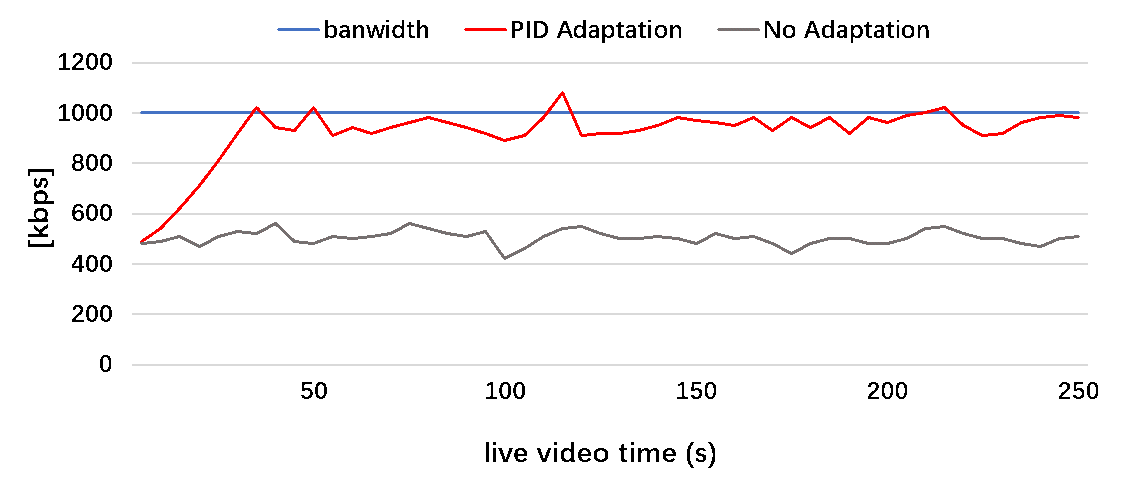
\includegraphics[width=0.8\textwidth]{clip/09-1.png}} \\
	\subfloat[长周期波动带宽的实验结果]{\label{fig:09-2}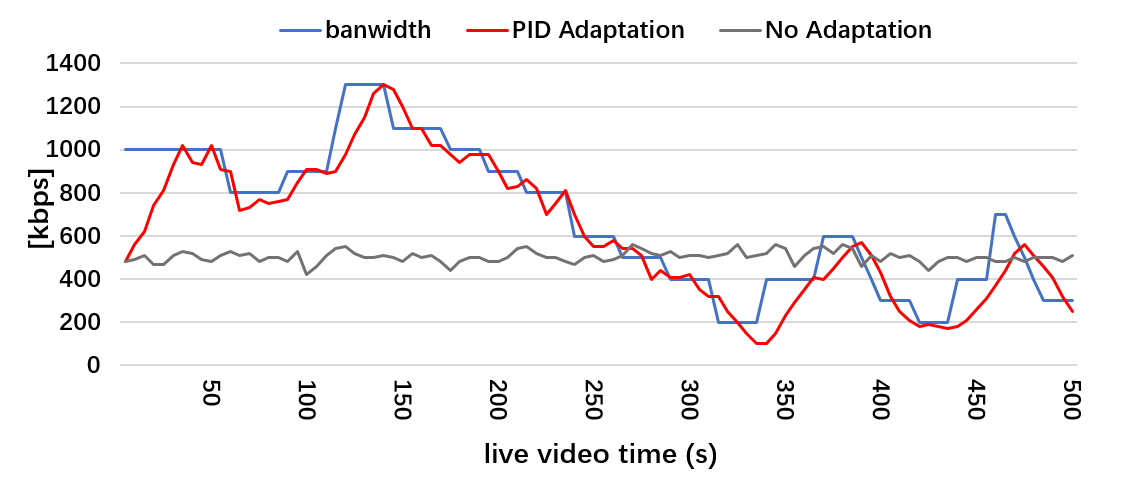
\includegraphics[width=0.8\textwidth]{clip/09-2.png}} \\
	\subfloat[短周期波动带宽的实验结果]{\label{fig:09-3}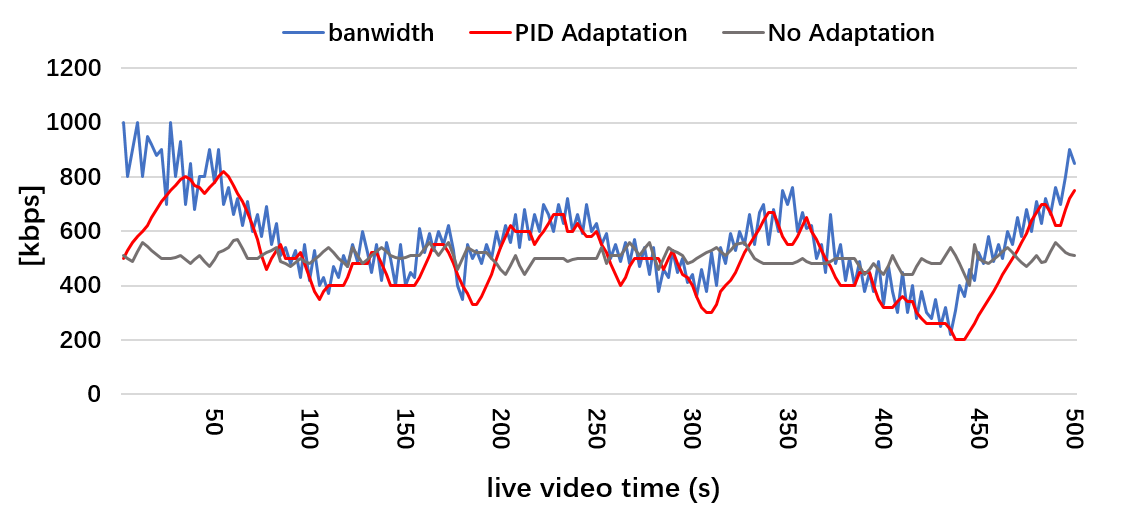
\includegraphics[width=0.8\textwidth]{clip/09-3.png}}
	\caption{直播系统在不同测试条件下码率随时间变化的情况}
	\label{fig:09}
\end{figure}

从图\ref{fig:09-1}中可以看出,我们提出的方法使得码率在35秒以内保持上升,直到趋近带宽。从图\ref{fig:09-2}和\ref{fig:09-3}可以看出,通过我们的方法进行的调整,在一个合理的延迟以内,码率和波动的带宽基本保持同步,而且对带宽的频繁变化做了一定的平滑。总之,加入PID码率自适应算法比不进行码率调整的直播效果有所改善。


\section{本章小结}

本章首先对PID控制器的基本思想做了简单介绍,然后将其用到了视频流媒体中的码率自适应问题中。在选择了合适的过程变量与控制目标之后,对通用PID模型稍作修改,得到了更加直观有效的基于比例的模型,并据此给出了码率自适应算法(又称为质量控制算法)。所提出的算法相比于其他算法不仅提高了所发送视频的平均质量,还降低了质量波动,取得了更好的平滑性。当流媒体服务器把最佳视频码流传送给用户后,在下一章中我们讨论如何对视频流的解码过程进行优化,以确保尽可能多的客户端设备能达到播放高清甚至超高清视频的条件。